\documentclass[11pt,a4paper]{article}

\usepackage{fullpage}
\usepackage[utf8]{inputenc}
\usepackage[russian]{babel}
\usepackage{graphicx}
\usepackage{float}
\usepackage[stable]{footmisc}
\usepackage{caption}
\usepackage{subcaption}
\usepackage{url}
\setcounter{section}{-1}

\setlength\parindent{0pt}

\title{Конспект по проектированию ПО \\ \vspace{2 mm} {\large v0.3}}
\date{}

\begin{document}
\maketitle
\tableofcontents

\section{Disclaimer}
Это конспект по курсу «Проектирование программного обеспечения», прочитанному year2011 на четвёртом курсе. Автор конспекта была на всех парах, на которых был и преподаватель\footnote{Дмитрий Юрьевич Кочелаев}, кроме одной (на которой, по счастливому стечению обстоятельств, лекции не было). В этом документе местами сказано больше, чем было на лекциях (так как он является жалкой попыткой автора подготовиться к сдаче зачёта), но местами — меньше (так как эти места были относительно лирическими отступлениями на лекциях, которые в общем и в целом вписываются в тему, но в ответе на вопрос смотрятся не к месту), так что его можно считать отрефакторенным конспектом, не покрытым тестами\footnote{Если вы не поняли последние пять слов, то поймёте после прочтения шестой главы.}. Дословная точность цитат не гарантируется, но никаких распятых мальчиков тут нет.

Конспект лежит по адресу \url{https://github.com/katyatitkova/software-design-outline}.

TODO: 
\begin{itemize}
\item вычитывание теми, кто был на парах;
\item недостающие картинки к паттернам;
\item дописать ещё про паттерны;
\item убрать пробелы в многослойной архитектуре.
\end{itemize}

\section{Порождающие паттерны\footnote{На самом деле, здесь почти всё взято из книжки.}}
Книжка по паттернам — конечно же, Банда Четырёх\footnote{Ralph Johnson, John Vlissides, Richard Helm, and Erich Gamma ``Design Patterns: Elements of Reusable Object-Oriented Software''}. Картинки здесь — с \url{http://www.oodesign.com}.
\subsection{Singleton}
Гарантирует, что у класса есть только один экземпляр, и предоставляет ему глобальную точку доступа.

\begin{figure}[H]
	\centering
	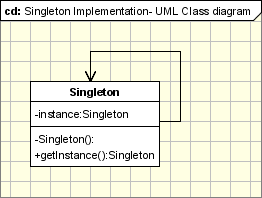
\includegraphics[width=200pt]{pics/singleton-pattern.png}
\end{figure}

\subsection{Pool\footnote{Нет в GoF.}}
Храним объекты готовыми к использованию: когда нужен, берём из пула (а не создаём), когда не нужен — возвращаем в пул (а не удаляем). Pool объектов никогда нельзя писать самому.

\begin{figure}[H]
	\centering
	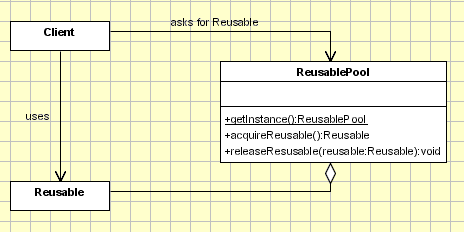
\includegraphics[width=300pt]{pics/objectpool-pattern.png}
\end{figure}

\subsection{Builder}
Отделяет конструирование сложного объекта от его представления: в результате одного и того же процесса конструирования могут получаться разные представления.

\begin{figure}[H]
	\centering
	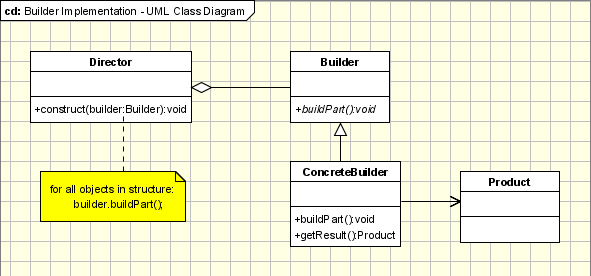
\includegraphics[width=350pt]{pics/builder-pattern.png}
\end{figure}

\subsection{Prototype}
Задаёт виды создаваемых объектов с помощью экземпляра-прототипа и создаёт новые объекты, копируя этот прототип.

Используем, когда нужно много одинаковых объектов: например, в текстовом редакторе отрендерили один раз букву и юзаем. А ещё существует извращённый прототип с наследованием.

\begin{figure}[H]
	\centering
	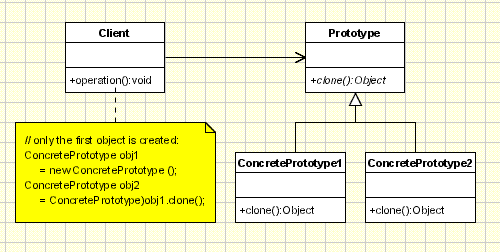
\includegraphics[width=300pt]{pics/prototype-pattern.png}
\end{figure}

\subsection{Factory Method}
Определяет интерфейс для создания объекта, но оставляет подклассам решение о том, какой класс инстанцировать. Позволяет делегировать инстанцирование подклассам.

\subsection{Abstract Factory}
Фабрика фабрик. Предоставляет интерфейс для создания семейств взаимосвязанных или взаимозависимых объектов, не специфицируя их конкретных классов.

\begin{figure}[H]
	\centering
	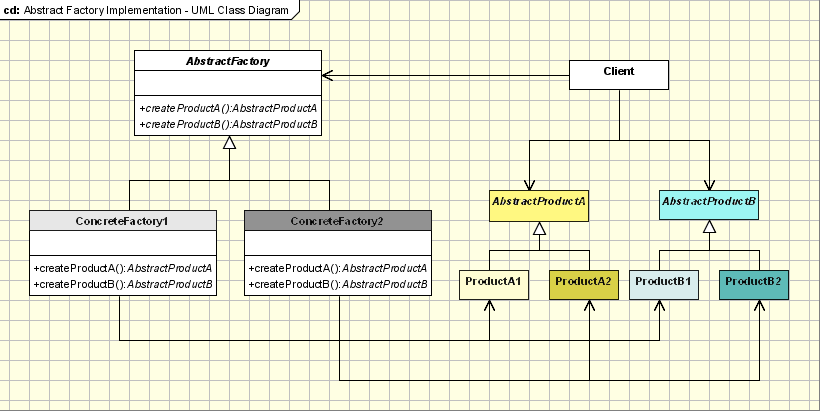
\includegraphics[width=450pt]{pics/abstract-factory-pattern.png}
\end{figure}

\section{Структурные паттерны\footnote{И тут тоже.}}
\subsection{Adapter}
Чтоб скрестить ежа с ужом: для юзания классов, не совместимых по интерфейсу.

\begin{figure}[H]
	\centering
	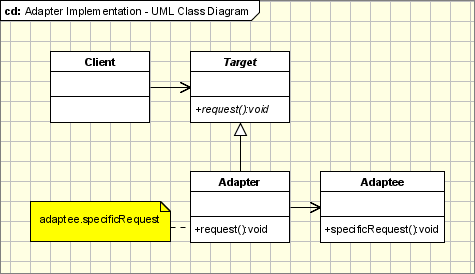
\includegraphics[width=300pt]{pics/adapter-pattern.png}
\end{figure}

\subsection{Bridge}
Отделяет абстракцию от её реализации так, чтобы их можно было изменять независимо.

\begin{figure}[H]
	\centering
	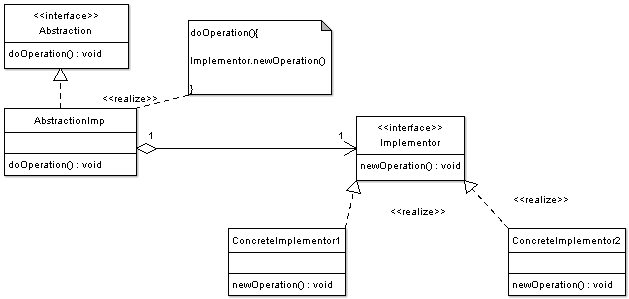
\includegraphics[width=400pt]{pics/bridge-pattern.png}
\end{figure}

\subsection{Composite}
Компонует объекты в древовидные структуры для представления иерархий часть-целое. Позволяет клиентам единообразно трактовать индивидуальные и составные объекты.

\begin{figure}[H]
	\centering
	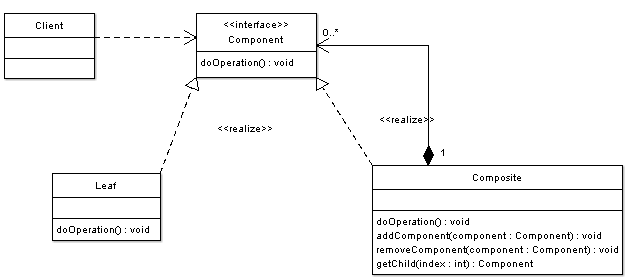
\includegraphics[width=400pt]{pics/composite-pattern.png}
\end{figure}

\subsection{Facade}
Предоставляет унифицированный интерфейс вместо набора интерфейсов подсистемы. Определяет интерфейс более высокого уровня для упрощения использования подсистемы. Если нет планов переписать, расширить, etc., то фасад не нужен.

\subsection{Decorator}
Динамически добавляет объекту новые обязанности. Является альтернативой порождению подклассов с целью расширения функциональности.

\begin{figure}[H]
	\centering
	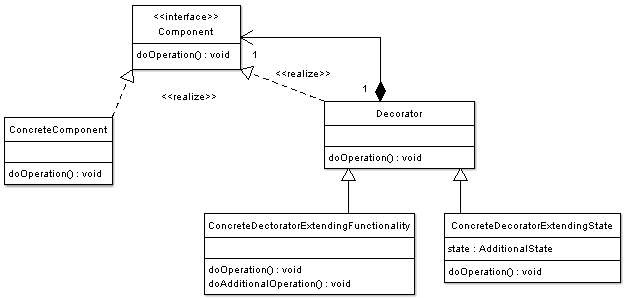
\includegraphics[width=400pt]{pics/decorator-pattern.png}
\end{figure}

\section{Многослойная архитектура}
\begin{figure}[H]
	\centering
	\begin{minipage}{.3\textwidth}
		\centering
		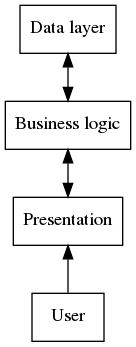
\includegraphics[width=70pt]{pics/layers.png}
		\captionof{figure}{Классика}
		\label{fig:layers}
	\end{minipage}%
	\begin{minipage}{.3\textwidth}
		\centering
		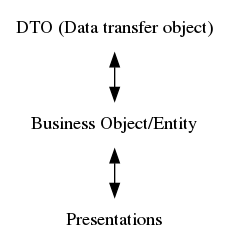
\includegraphics[width=130pt]{pics/dto.png}
		\captionof{figure}{1 layer — 1 object}
		\label{fig:dto}
	\end{minipage}
	\begin{minipage}{.35\textwidth}
		\centering
		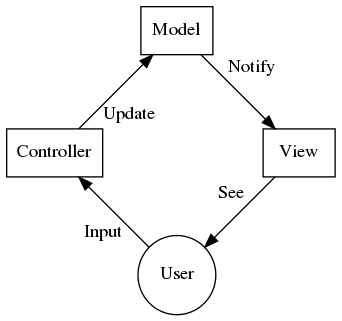
\includegraphics[width=180pt]{pics/mvc.png}
		\captionof{figure}{MVC}
		\label{fig:dto}
	\end{minipage}
\end{figure}

Казалось бы, по классической картинке всё понятно. Business logic может разрастаться вертикально.

\begin{enumerate}
\item 1 layer — 1 object

DTO — это объект, который используется для передачи данных между слоями. Сокращает количество запросов, которые обычно дороги.
\item All layers — 1 object\footnote{Кажется, никто из тех, кто ходил, не помнит, что это :( Читающий, если ты помнишь — допиши сам или расскажи Титковой!}
\end{enumerate}

Дальше было что-то про ORM.

MVC (Model-view-controller)

\section{Inversion of Control \& Dependency Injection}
Реализация принципа ``Don't call us, we'll call you''. Например, была консольная программка, которая складывала числа, которая говорила: «введите a», «введите b» (то есть программа говорила, что делать), а теперь — программка с полями для ввода и кнопкой calculate, где можно править значения в любом порядке (то есть мы управляем).

IoC нужен, чтобы:
\begin{enumerate}
\item разделить функциональность между этапами запуска и реализации;
\item разграничить: каждый модуль занимается только своей задачей, физически нельзя залезть в чужое;
\item дать модулям полагаться на контракты.
\end{enumerate}

Способы реализации:
\begin{enumerate}
\item Dependency injection — передаём dependency (сервис) dependent object'у (клиенту), то есть сервис становится частью клиента. Весело дебагать. Из интерфейса понятно, что и как у нас с клиентом.
\item Service locator — сами ищем сервис, который отвечает за нашу функциональность. Гораздо проще реализовать (в примитиве — HashMap), так как перекладывает часть логики на клиента, но значительно сложнее протестировать. В использовании зависим от интерфейса.
\end{enumerate}

Подходы к конфигурации DI:
\begin{enumerate}
\item inline (прямо в коде);
\item configs (xml, json…);
\item annotation.
\end{enumerate}

DI ещё даёт возможность использовать прокси и аспекты.

AOP (aspect-oriented programming)

Аспект — некий модуль, который реализует сквозную функциональность (функциональность, которую нельзя выделить в отдельные сущности; её реализация распределена по различным модулям программы).

Advice (совет) — дополнительная функциональность, которую хотим внести в код.

Injection point (join point) — то место, где следует применить advice.

\section{Message Queue}
Message queue — способ подружить два и более приложений. До этого были CORBA\footnote{Common Object Request Broker Architecture}, OLE\footnote{Object Linking and Embedding}, WS\footnote{Web Service(?)}.

Пример: рассылаем смс о транзакциях в банке.

\begin{figure}[H]
	\centering
	\begin{minipage}{.5\textwidth}
		\centering
		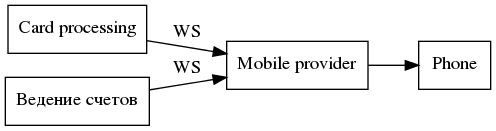
\includegraphics[width=200pt]{pics/ws.png}
		\captionof{figure}{Плохая схема}
		\label{fig:ws}
	\end{minipage}%
	\begin{minipage}{.5\textwidth}
		\centering
		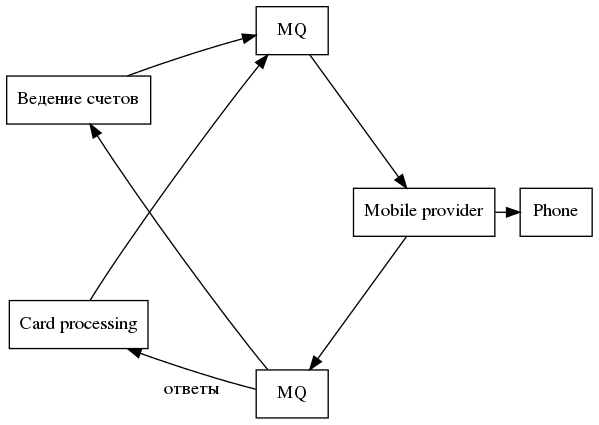
\includegraphics[width=230pt]{pics/mq.png}
		\captionof{figure}{Хорошая схема}
		\label{fig:mq}
	\end{minipage}
\end{figure}

У нас есть какая-то пропускная способность для отправки смсок. Первого числа всем начислили зарплату, пошёл поток смсок. При плохой схеме у нас висят транзакции, по которым ещё не отправились. При хорошей мы завершили транзакцию, отправив смску в очередь.

Очередь должна уметь восстанавливаться, поэтому мы делаем их три. Ответ «ок» на клиенте, когда мы положили сообщение во все очереди. Зачем три? Если одна умерла, то по тому, есть ли сосед, понимаем, мы умерли или не мы\footnote{«Кто не смотрел ``Шестое чувство'': это был спойлер»}

Гарантии доставки:
\begin{itemize}
\item at least once — доставляем минимум один раз, чтоб гарантированно получить ответ;
\item at most once — доставляем максимум один раз (выполнить операцию дважды хуже, чем не выполнить вообще).
\end{itemize}

\begin{figure}[H]
	\centering
	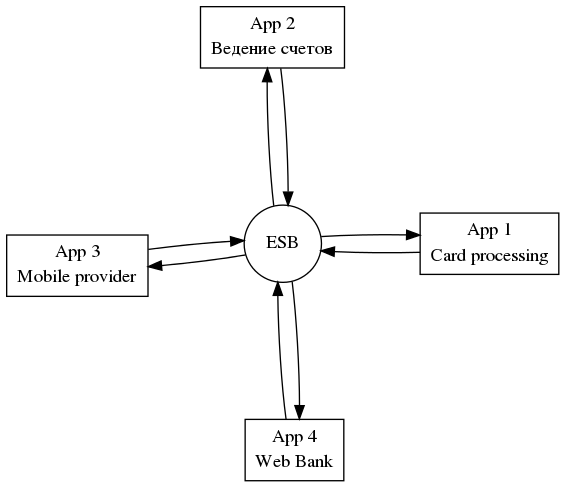
\includegraphics[width=200pt]{pics/bus.png}
	\caption{(Enterprise) Service Bus. Стрелочки чаще всего — очереди}
\end{figure}

В очередях плохо хранить большие сообщения, поэтому обычно header хранят в очереди, а binary data — в file storage.

\section{Рефакторинг}
По рефакторингу есть классическа книжка Фаулера\footnote{Martin Fowler ``Refactoring: Improving the Design of Existing Code''}. ДК говорит, что Фаулер считает, что «жить без рефакторинга так же сложно, как без Крыма». И советует для общего образования пролистать оглавление, а если есть куча свободного времени — почитать. Но от него хорошо засыпается\footnote{…и поэтому автор только пролистала. Там действительно разобраны довольно очевидные проблемы с довольно очевидными путями решения.}.

Рефакторить можно код, структуру БД, интерфейсы.

\subsection{Рефакторинг кода}
Preconditions для рефакторинга кода с точки зрения Фаулера (не ДК):
\begin{itemize}
\item добавляется новая функциональность;
\item исправление ошибок («как если криво висела картина, а мы заодно обои переклеили»);
\item изучение кода («самое страшное», «как если висит полочка, вытащили её, снова переклеили обои, пролили клей на паркет, переложили его, а попутно сломали кафель в ванной…»)
\end{itemize}

Да, «рефакторинг — как ремонт». Вообще, «первые два пункта имеют право на жизнь», а «новая функциональность без рефакторинга — как балконы в Молдавии»\footnote{Дальше был рассказ ДК о том, что в Молдавии любят достраивать балконы вперёд, причём балконы третьего этажа опираются на достроенные балконы второго и так далее.}, но «надо было переклеить одно полотнище — не надо перекладывать кафель у соседей».

Для рефакторинга нужен хороший coverage тестами, но тесты-то тоже переделаются…

Test-driven development, с точки зрения ДК, гиблый метод. «Есть тесты, и нет ничего. Обычно в этот момент сдавать надо». Раз сразу всё обложили тестами, то придумали и интерфейс, а он всё равно десять раз перепишется, пока будем писать код.

Кстати, выкинуть старое, написать новое — не рефакторинг.

Если у нас coverage тестами $95\%$, то можно не рефакторить функцию на 15 экранов. А развернуть цикл иногда ок: например, если это цикл до $4$, занимающийся получением byte'ов из int'а, так понятнее будет.

Советы ДК по поводу рефакторинга кода:
\begin{itemize}
\item не рефакторить просто так;
\item рефакторить, только если обложили всё тестами;
\item сразу писать так, чтобы не рефакторить;
\item полезный рефакторинг — в процессе написания.
\end{itemize}

\subsection{Рефакторинг БД}
Рефакторинг БД и интерфейсов — занятие мрачное и неблагодарное. Принципиальное отличие рефакторинга БД от рефакторинга кода — нет тестов для структуры БД, у всех всё может работать, но неправильно. Добавить новую колонку не страшно, обычно не ломает старое, а вот расширение поля — ой.

Советы от ДК:
\begin{itemize}
\item пытаться писать тесты на БД;
\item спроектировать сразу хорошо.
\end{itemize}

\subsection{Рефакторинг интерфейсов}
После рефакторинга интерфейса все пользователи нашей библиотеки нас люто ненавидят. Правильно делать так: 

\begin{enumerate}
\item выкатываем новый API в sandbox (в котором работают оба, можно их посравнивать между собой);
\item в продакшне работают оба API (причём хорошо сделать такой ключ, что все, кто получил его после выхода нового, не могут использовать старый);
\item можно убить старый (отвалятся примерно $15\%$ приложений, использующих его, из них $50\%$ ничего не заметят, $15\%$ напишут гневное письмо, но ничего не сделают, остальные как-то приспособятся).
\end{enumerate}

А за рефакторинг как самоцель надо бить.

\section{Параллельные транзакции}
Перенесёмся в доисторические времена, когда VCS не было, но программисты уже существовали. Был у них шареный диск, общая папка, общие исходники. И открыл первый программист файл, и писал в него целый день. А второй открыл на два часа позже, что-то исправил, и сохранил. И первый сохранил. Но в результате у нас lost changes — никто ничего не сделал! Так вот, эти чуваки — два потока с параллельными транзакциями.

Ещё пример. Продолжаем работать, считаем замечательную метрику кода: количество классов в каждом пакете. Просто проходим по директориям и считаем. Пусть у нас есть директория \texttt{A} с классами \texttt{A1} и \texttt{A2} и директория \texttt{B} с \texttt{B1}, \texttt{B2}, \texttt{B3}, \texttt{B4}. Насчитали два класса в \texttt{A} и ушли на перекур. В это время пришёл второй чувак, создал \texttt{A3} и удалил \texttt{B3} и \texttt{B4}. Пришли, досчитали, что в \texttt{B} два класса, «сложили 2 + 2 на js, получили 22, отдаём отчёт начальству». Но проблема в том, что у нас ни в какой момент не было четырёх классов. Это — несогласованные чтения (inconsistent read).

Это лишь маленькие проблемы, которые возникают при работе без попыток что-то урегулировать. «Тут хуже, чем дикий Запад. Прям Мытищи какие-то».

\subsection{Как бороться с тем, что одновременно меняем одни и те же ресурсы?}
\begin{enumerate}
\item Isolate (изолированность транзакций): захотели поработать с файлом — делаем lock файла, «ушли, забыли разлочить, заболели на две недели, уехали в отпуск ещё на три, попутно нас прокляли»;
\item Immutability: большое количество файлов, которые неизменяемы;
\item Общаемся с данными только read-only.
\end{enumerate}

Если бы всё было read-only, проблем бы не было.

\subsection{Пессимистические и оптимистические блокировки}
Пессимистическая — только бы ничего не случилось. Лочим всегда, даже если не факт, что случится конфликт: залочили ресурс, желая только прочесть из него, и другой чувак не сможет получить доступ даже для чтения. Из плюсов — конфликты никогда не случаются, всё можно делать в автоматическом режиме. Минусы — снижается производительность, параллелизм резко падает.

Оптимистическая — кто первый встал, того и тапки. Параллелизм ок, но приходится разрешать конфликты.

Выбираем между ними по следующим критериям:
\begin{itemize}
\item частота доступа;
\item длительность доступа;
\item возможность разрешения конфликтов.
\end{itemize}

В VCS оптимистические. В каком-нибудь биллинге — пессимистические, ибо некому разрешать конфликы, изменения короткие и их много.

Но! Пусть есть три класса.

\begin{figure}[H]
	\centering
	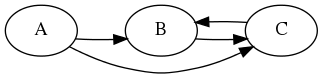
\includegraphics[width=200pt]{pics/locks.png}
\end{figure}

Стрелочками обозначены зависимости между ними. Возьмём пессимистическую блокировку: один чувак на A, другой — на B. Не столкнутся по блокировке, но, может быть, ничего работать не будет. А всё потому, что блокировку надо накладывать на все ресурсы, от которых мы зависим.

Есть два типа блокировок: exclusive и shared. Вторая — это когда залочить надо, но менять мы не собираемся, тогда несколько пользователей могут прочитать этот ресурс.

Но даже с этим возможны проблемы, а именно — deadlocks. Они появляются, когда мы, имея shared блокировку, хотим получить exclusive, или «получаем больше блокир.» TODO распарсить. Разрешаем выбором жертвы, которую надо убить: по таймауту или по принципу «ты мне не нравишься».

Впрочем, сам по себе дедлок не страшен — например, в биллинге всё просто распределится на другие потоки. Если возможны дедлоки, то приложение должно иметь это в виду.

\subsection{Основные свойства транзакции}
\begin{itemize}
\item \textbf{A}tomicity — транзакция или вся целиком выполняется, или вся целиком не выполняется;
\item \textbf{C}onsistency — каждая транзакция приводит к валидным данным;
\item \textbf{I}solation — транзакция не может работать с ресурсами транзакций, которые ещё не завершены;
\item \textbf{D}urability — результаты завершённых транзакций не будут утеряны.
\end{itemize}

Эти свойства далеко не везде выполняются.
\begin{enumerate}
\item Phantom objects — из-за второй транзакции в нашей появляются новые объекты;
\item Unrepeatable reads — выполняем чтение, в соседней транзакции поменяли, снова выполняем чтение;
\item Garbage reads — видим данные из транзакций, которые ещё не завершились (уточнить).
\end{enumerate}

Транзакции по соблюдению этих правил бывают \textit{посмотреть в курсе БД и распарсить записи в тетрадке}.

\section{Сессии}
Анонимный пользователь Михаил\footnote{«Если мы параноики, мы не подключены к интернету»}, отключив куки и включив порно-режим, изучает книжки на амазоне. Каждый запрос не зависит от предыдущего из-за параноидальности, это — сессия без состояния (stateless session). Некоторое время назад большая часть была такой.

Теперь Михаил ходит по сайту, не залогинившись, и везде есть плашечка «вы недавно посмотрели». Это — statefull session, сессия с состоянием.

И, наконец, он решил что-то купить. Это тоже statefull (но action, а не view, как предыдущие? уточнить).

Как сохранить состояние? Три варианта:
\begin{enumerate}
\item самый простой — на стороне клиента (cookies, …) (client-side);
\item server-side;
\item database.
\end{enumerate}

Если всё на клиенте, для сервера в каждом запросе вся инфа, что ему нужна. Должна быть mutable с точки зрения сервера. Server-side — у клиента session\_id, он передаёт его серверу; guid\footnote{Globally Unique Identifier} гарантированно уникальный и считается относительно дорого. DB — ???

Что будет, если Михаил вдруг закроет ноут? client-side — ничего, просто сессия заэкспайрится когда-то. server-side — надо будет почистить память (это не persistent storage, так что может и почистить память). DB — точно надо подчистить.

С точки зрения durability в случае отказа база всегда есть, сервер может того, как и клиент. В базе всё ок, что не умерло, всё подняли из базы. А если клиент умер, то надо подчистить его контекст на сервере.

\subsection{Кластеризация}
У нас есть приложение для просмотра котиков, у нас в 10 раз больше подписчиков, чем у инстаграма, мы в десять раз убыточнее, нас покупают в десять раз дороже. Хотим кластеризоваться. Первый вариант — а-ля сбер: берём самую мощную IBM-железку в мире (таких всего 3 инсталляции), хотим туда что-то от оракла, и оказывается, что это единственная инсталляция и ребята из оракла не знают, что делать. Второй вариант — увеличиваем число серверов, но каждый запрос от клиента проходит через Load Balancer (nginx, apache…). Рассматриваем, понятное дело, его.

Если всё на клиенте, то проблем нет — всё своё ношу с собой. Иначе варианты:
\begin{itemize}
\item sticky session — в рамках одной сессии пользователь всегда на одном и том же сервере. Проблемы: может быть \textit{(кто, что?)} простой одних серверов при перегруженности других, а если сервер сдохнет, сессия может потеряться.
\item round-robin — $n$-ая таска идёт $n \ mod \ M$-ому серверу, где $M$ — число серверов.
\end{itemize}

Боремся с перегруженностью: session transfer. Сервера всё же взаимосвязаны и умеют обмениваться сессиями. Только надо ещё уведомить LB.

Боремся со смертью сервера: distributed session (но надо реплицировать все сессии, а это дорого), distributed memory cache (получаем информацию о сессии из кэша, которые отделно от серверов).

\section{Распределённые вычисления}
Люди раньше, начитавшись про корбу и RMI, все объекты (client, address, contract, subscriptions…) клали по разным серверам. Вырос контракт — нарастили ноду. Но на запрос между нодами тратится очень много времени, да ещё и стараемся не вдаваться в детали: хотим данные об адресе — получаем вообще весь адрес и разбираем его у себя локально.

Локализация remote-интерфейсов:
\begin{enumerate}
\item фасады;
\item ленивая инициализация объектов, которые пришли удалённо;
\item data transfer object.
\end{enumerate}

Бывают ещё SOAP, json-запросы over-http, абстрактные сериализаторы типа protobuff'а.

Этот раздел был в конце лекции, и какой-то он странный

\section{Release Management\footnote{«Лучше бы про что-то другое поговорил»}}
Как всё обычно делается? «фигак, фигак и в продакшн»\footnote{Из-за присутствия автора на лекции было сказано именно так.}

Была у нас общая папка для хранения исходников, получились проблемы, как уже было рассказано ранее, перешли к version control. Многие используют его как ту папку — одна большая толстая ветка. Было CVS — были и бранчи, и теги, а каждый релиз — склеивание бранчей на денёк. Потом был SVN, стало немного гуманнее в этом. Потом появился приличный VC.

Есть два пути: побранчуемся и склеимся, потом в продакшн, или continuous delivery\footnote{«Надо потом хорошо стереть, а то скажут, что я вас тут плохому учу». На доске: «Continuous Delivery (не лучший вариант, но, если очень надо, то можно!)»}.

CD — это полный-полный Agile в худшем понимании этого слова.

[тут, возможно, будут картинки]

Вывод из картинок: бранчи должны быть короткие.

Создавать новые бранчи можно по принципам:
\begin{itemize}
\item Branch per Release — был популярен в централизованных VC. Все работают над тем, что идёт в продакшн, но все работают над одним и тем же кодом;
\item Branch per Task;
\item Promotional Branch (выпустили 1.1, выпустили 1.2, и тут оказалось, что надо пропатчить 1.1, и так и идёт тысяча ужасных ответвлений);
\item Branch per Component;
\item Branch per OS.
\end{itemize}

Накладные расходы от бранчевания: надо мёржиться, больше тестирования.

Антипаттерны бранчевания:
\begin{itemize}
\item боязнь мёржиться;
\item сразу мёржить в мастер (много времени на мёрж, высока вероятность, что код какой-то странный);
\item бесконечные бранчи;
\item мёрж не в ту сторону (из 1.2 перенесли функциональность в 1.1, потому что какой-то клиент обновляться не хочет);
\item отдельные ветки для кучи маленьких изменений (pull request);
\item каскадные бранчи (есть бранч на 1.1, от него на 1.2 и так далее, а вообще есть бранч на 2.1…);
\item временные бранчи;
\item нестабильные бранчи (сбранчевались, пока код не работает);
\item бранчи на члена команды.

«Рано или поздно вы с чем-то из этого столкнётесь».
\end{itemize}
\end{document}